\chapter{Vision Architectures}
\label{chap:vision_architectures}

\begin{tldr}
This chapter covers vision architectures beyond basic CNNs: Vision Transformers (ViT), hierarchical transformers (Swin), object detection (YOLO, DETR), and segmentation (U-Net, Mask R-CNN, SAM). Understanding the trade-offs between CNNs and Transformers, and when to use each detection/segmentation approach, is crucial for vision-related interview questions.
\end{tldr}

\section{CNN Fundamentals Review}
\label{sec:cnn_review}

\subsection{Inductive Biases of CNNs}

\begin{enumerate}
    \item \textbf{Locality}: Neurons connect only to local regions
    \item \textbf{Translation equivariance}: Same filter applied everywhere
    \item \textbf{Weight sharing}: Same parameters across spatial locations
\end{enumerate}

These biases make CNNs data-efficient for vision but limit modeling of global context.

\subsection{Receptive Field}

\textbf{Receptive Field.} The region in the input that affects a particular activation.

For a stack of $L$ layers with kernel size $k$ and stride 1:
\begin{equation}
RF = 1 + L \times (k - 1)
\end{equation}

With dilated convolutions (dilation $d$):
\begin{equation}
\text{effective kernel} = k + (k-1)(d-1)
\end{equation}

\subsection{CNN Architecture Evolution}

\begin{table}[H]
\centering
\caption{CNN architecture evolution}
\begin{tabularx}{\textwidth}{lrXl}
\toprule
\textbf{Model} & \textbf{Year} & \textbf{Key Innovation} & \textbf{Top-1 Acc} \\
\midrule
AlexNet & 2012 & ReLU, dropout, GPU training & 63.3\% \\
VGG & 2014 & Small (3×3) filters, depth & 74.4\% \\
GoogLeNet & 2014 & Inception modules, 1×1 conv & 74.8\% \\
ResNet & 2015 & Skip connections, very deep & 78.6\% \\
DenseNet & 2017 & Dense connections & 79.2\% \\
EfficientNet & 2019 & Compound scaling & 84.4\% \\
ConvNeXt & 2022 & Modernized ResNet & 87.8\% \\
\bottomrule
\end{tabularx}
\end{table}

%==============================================================================
\section{Vision Transformer (ViT)}
\label{sec:vit}
%==============================================================================

\subsection{Architecture}

\begin{figure}[H]
\centering
\begin{tikzpicture}[
    node distance=0.5cm,
    box/.style={rectangle, draw, minimum width=1.2cm, minimum height=0.6cm, rounded corners, font=\small, align=center}
]
    % Image
    \node (img) {Image};
    
    % Patches
    \node[box, fill=yellow!20, right=0.8cm of img] (patch) {Patch\\Embed};
    
    % Position embedding
    \node[box, fill=lightgreen, right=0.8cm of patch] (pos) {+ Pos\\Embed};
    
    % CLS token
    \node[above=0.3cm of pos, font=\small] (cls) {+ {[CLS]}};
    
    % Transformer
    \node[box, fill=lightblue, right=0.8cm of pos, minimum height=1.5cm] (trans) {Transformer\\Encoder\\$\times$L};
    
    % Output
    \node[box, fill=orange!30, right=0.8cm of trans] (head) {MLP\\Head};
    
    \node[right=0.5cm of head] (out) {Class};
    
    % Edges
    \draw[->] (img) -- (patch);
    \draw[->] (patch) -- (pos);
    \draw[->] (cls) -- (pos);
    \draw[->] (pos) -- (trans);
    \draw[->] (trans) -- (head);
    \draw[->] (head) -- (out);
\end{tikzpicture}
\caption{Vision Transformer (ViT) architecture.}
\end{figure}

\subsection{Patch Embedding}

Split image into non-overlapping patches and linearly project:
\begin{equation}
\vz_0 = [\vx_{cls}; \vx_p^1\mE; \vx_p^2\mE; \ldots; \vx_p^N\mE] + \mE_{pos}
\end{equation}

where:
\begin{itemize}
    \item $\vx_p^i \in \R^{P^2 \cdot C}$ is flattened patch
    \item $\mE \in \R^{(P^2 \cdot C) \times D}$ is patch embedding projection
    \item $P$ = patch size (typically 16)
    \item $N = \frac{H \cdot W}{P^2}$ = number of patches
\end{itemize}

\subsection{ViT vs. CNN Trade-offs}

\begin{table}[H]
\centering
\caption{ViT vs. CNN comparison}
\begin{tabularx}{\textwidth}{lXX}
\toprule
\textbf{Aspect} & \textbf{ViT} & \textbf{CNN} \\
\midrule
Inductive bias & Minimal (learns from data) & Strong (locality, translation) \\
Data efficiency & Needs large data (JFT-300M) & Works with moderate data \\
Global context & From layer 1 & Requires depth \\
Computational scaling & Better at scale & Better at small scale \\
Small objects & Can struggle (patch size) & Better local detail \\
\bottomrule
\end{tabularx}
\end{table}

\subsection{ViT Variants}

\begin{table}[H]
\centering
\caption{ViT model sizes}
\begin{tabular}{lrrrr}
\toprule
\textbf{Model} & \textbf{Layers} & \textbf{Hidden} & \textbf{Heads} & \textbf{Params} \\
\midrule
ViT-B/16 & 12 & 768 & 12 & 86M \\
ViT-L/16 & 24 & 1024 & 16 & 307M \\
ViT-H/14 & 32 & 1280 & 16 & 632M \\
\bottomrule
\end{tabular}
\end{table}

%==============================================================================
\section{Hierarchical Vision Transformers}
\label{sec:hierarchical_vit}
%==============================================================================

\subsection{Swin Transformer}

\textbf{Key innovations}:
\begin{enumerate}
    \item \textbf{Hierarchical feature maps}: Progressive downsampling like CNNs
    \item \textbf{Shifted windows}: Local attention within windows, shifted for cross-window connection
    \item \textbf{Linear complexity}: $O(n)$ vs. $O(n^2)$ for global attention
\end{enumerate}

\begin{figure}[H]
\centering
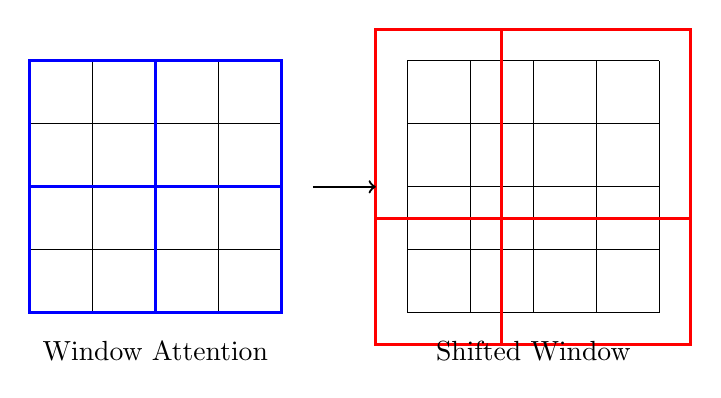
\begin{tikzpicture}[scale=0.8]
    % Regular windows
    \begin{scope}[shift={(0,0)}]
        \draw[step=1] (0,0) grid (4,4);
        \draw[very thick, blue] (0,0) rectangle (2,2);
        \draw[very thick, blue] (2,0) rectangle (4,2);
        \draw[very thick, blue] (0,2) rectangle (2,4);
        \draw[very thick, blue] (2,2) rectangle (4,4);
        \node[below] at (2, -0.3) {Window Attention};
    \end{scope}
    
    % Shifted windows
    \begin{scope}[shift={(6,0)}]
        \draw[step=1] (0,0) grid (4,4);
        \draw[very thick, red] (-0.5,-0.5) rectangle (1.5,1.5);
        \draw[very thick, red] (1.5,-0.5) rectangle (4.5,1.5);
        \draw[very thick, red] (-0.5,1.5) rectangle (1.5,4.5);
        \draw[very thick, red] (1.5,1.5) rectangle (4.5,4.5);
        \node[below] at (2, -0.3) {Shifted Window};
    \end{scope}
    
    \draw[->, thick] (4.5, 2) -- (5.5, 2);
\end{tikzpicture}
\caption{Swin Transformer: Regular windows followed by shifted windows enable cross-window connections.}
\end{figure}

\subsection{Feature Pyramid from Swin}

Like CNNs, Swin produces multi-scale features:
\begin{itemize}
    \item Stage 1: $\frac{H}{4} \times \frac{W}{4}$, 96 channels
    \item Stage 2: $\frac{H}{8} \times \frac{W}{8}$, 192 channels
    \item Stage 3: $\frac{H}{16} \times \frac{W}{16}$, 384 channels
    \item Stage 4: $\frac{H}{32} \times \frac{W}{32}$, 768 channels
\end{itemize}

This makes Swin directly usable for detection and segmentation.

%==============================================================================
\section{Object Detection}
\label{sec:object_detection}
%==============================================================================

\subsection{Detection Paradigms}

\begin{figure}[H]
\centering
\begin{tikzpicture}[
    node distance=1.5cm,
    box/.style={rectangle, draw, rounded corners, minimum width=2.5cm, minimum height=0.8cm, fill=lightblue, font=\small}
]
    \node[box] (twostage) {Two-Stage};
    \node[box, right=3cm of twostage] (onestage) {One-Stage};
    \node[box, right=3cm of onestage] (transformer) {Transformer};
    
    \node[below=0.5cm of twostage, font=\small] {Faster R-CNN};
    \node[below=0.5cm of onestage, font=\small] {YOLO, SSD};
    \node[below=0.5cm of transformer, font=\small] {DETR};
    
    \node[below=1cm of twostage, font=\tiny, text width=2.5cm, align=center] {Region proposals\\then classify};
    \node[below=1cm of onestage, font=\tiny, text width=2.5cm, align=center] {Direct prediction\\from feature map};
    \node[below=1cm of transformer, font=\tiny, text width=2.5cm, align=center] {Set prediction\\with attention};
\end{tikzpicture}
\caption{Object detection paradigms.}
\end{figure}

\subsection{Two-Stage Detectors (Faster R-CNN)}

\begin{enumerate}
    \item \textbf{Backbone}: Extract features (ResNet, etc.)
    \item \textbf{RPN (Region Proposal Network)}: Propose candidate boxes
    \item \textbf{RoI Pooling/Align}: Extract features for each proposal
    \item \textbf{Classification + Regression}: Classify and refine boxes
\end{enumerate}

\textbf{Pros}: High accuracy, well-understood
\textbf{Cons}: Slower, complex pipeline

\subsection{One-Stage Detectors}

\subsubsection{YOLO (You Only Look Once)}

\begin{itemize}
    \item Divide image into grid
    \item Each cell predicts $B$ boxes + confidences + class probs
    \item Single forward pass
\end{itemize}

\textbf{Evolution}: YOLOv1 → v2 → v3 → v4 → v5 → v8 (continuous improvements)

\subsubsection{SSD (Single Shot Detector)}

\begin{itemize}
    \item Multi-scale feature maps
    \item Predictions at multiple scales
    \item Default boxes (anchors) at each location
\end{itemize}

\subsubsection{RetinaNet}

\textbf{Key innovation}: Focal loss to handle class imbalance
\begin{equation}
FL(p_t) = -\alpha_t (1-p_t)^\gamma \log(p_t)
\end{equation}

\subsection{DETR (Detection Transformer)}

\textbf{Key innovations}:
\begin{enumerate}
    \item \textbf{Set prediction}: Output fixed set of predictions, no NMS needed
    \item \textbf{Bipartite matching}: Hungarian algorithm to match predictions to GT
    \item \textbf{Object queries}: Learned queries attend to image features
\end{enumerate}

\begin{equation}
\mathcal{L} = \sum_{i=1}^{N} [\lambda_{cls} \mathcal{L}_{cls}(c_i, \hat{c}_{\sigma(i)}) + \lambda_{box} \mathcal{L}_{box}(b_i, \hat{b}_{\sigma(i)})]
\end{equation}

where $\sigma$ is the optimal assignment from Hungarian matching.

\subsection{Detection Architecture Selection}

\begin{table}[H]
\centering
\caption{Detection architecture selection}
\begin{tabularx}{\textwidth}{lXX}
\toprule
\textbf{Requirement} & \textbf{Recommended} & \textbf{Reason} \\
\midrule
Real-time (30+ FPS) & YOLOv8, YOLOv5 & Speed optimized \\
Highest accuracy & DETR variants, Cascade R-CNN & Best performance \\
Small objects & Faster R-CNN + FPN & Multi-scale features \\
Simple pipeline & DETR & End-to-end, no NMS \\
Edge deployment & YOLOv8-nano & Efficient \\
\bottomrule
\end{tabularx}
\end{table}

%==============================================================================
\section{Semantic Segmentation}
\label{sec:semantic_segmentation}
%==============================================================================

\subsection{Task Definition}

Assign a class label to every pixel in the image.

\subsection{Key Architectures}

\subsubsection{FCN (Fully Convolutional Networks)}

\begin{itemize}
    \item Replace FC layers with 1×1 convolutions
    \item Upsample to input resolution
    \item Skip connections from encoder
\end{itemize}

\subsubsection{U-Net}

\begin{figure}[H]
\centering
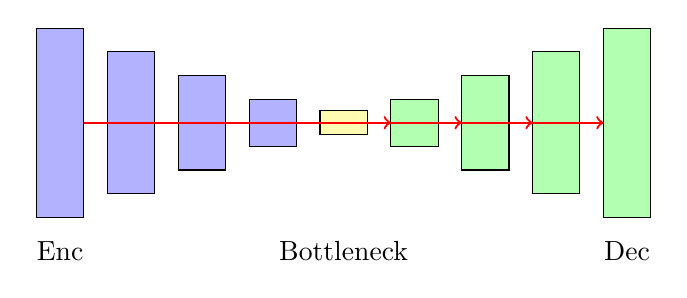
\begin{tikzpicture}[scale=0.6]
    % Encoder
    \draw[fill=blue!30] (0,0) rectangle (1,4);
    \draw[fill=blue!30] (1.5,0.5) rectangle (2.5,3.5);
    \draw[fill=blue!30] (3,1) rectangle (4,3);
    \draw[fill=blue!30] (4.5,1.5) rectangle (5.5,2.5);
    
    % Bottleneck
    \draw[fill=yellow!30] (6,1.75) rectangle (7,2.25);
    
    % Decoder
    \draw[fill=green!30] (7.5,1.5) rectangle (8.5,2.5);
    \draw[fill=green!30] (9,1) rectangle (10,3);
    \draw[fill=green!30] (10.5,0.5) rectangle (11.5,3.5);
    \draw[fill=green!30] (12,0) rectangle (13,4);
    
    % Skip connections
    \draw[->, thick, red] (1,2) -- (12,2);
    \draw[->, thick, red] (2.5,2) -- (10.5,2);
    \draw[->, thick, red] (4,2) -- (9,2);
    \draw[->, thick, red] (5.5,2) -- (7.5,2);
    
    % Labels
    \node[below] at (0.5, -0.3) {Enc};
    \node[below] at (6.5, -0.3) {Bottleneck};
    \node[below] at (12.5, -0.3) {Dec};
\end{tikzpicture}
\caption{U-Net architecture with skip connections.}
\end{figure}

\textbf{Key features}:
\begin{itemize}
    \item Symmetric encoder-decoder
    \item Skip connections preserve spatial detail
    \item Excellent for medical imaging
\end{itemize}

\subsubsection{DeepLab}

\textbf{Innovations}:
\begin{enumerate}
    \item \textbf{Atrous (dilated) convolution}: Larger receptive field without downsampling
    \item \textbf{ASPP}: Atrous Spatial Pyramid Pooling for multi-scale
    \item \textbf{CRF}: Conditional Random Field for boundary refinement
\end{enumerate}

%==============================================================================
\section{Instance Segmentation}
\label{sec:instance_segmentation}
%==============================================================================

\subsection{Task Definition}

Detect individual objects AND segment each instance separately.

\subsection{Mask R-CNN}

Extension of Faster R-CNN:
\begin{enumerate}
    \item Everything in Faster R-CNN
    \item + Mask head: Predict binary mask for each RoI
    \item RoI Align (not RoI Pool) for better spatial alignment
\end{enumerate}

\begin{equation}
\mathcal{L} = \mathcal{L}_{cls} + \mathcal{L}_{box} + \mathcal{L}_{mask}
\end{equation}

\subsection{SAM (Segment Anything Model)}

\textbf{Foundation model for segmentation}:
\begin{itemize}
    \item Trained on 11M images, 1B masks
    \item Promptable: Point, box, or text prompts
    \item Zero-shot transfer to new domains
\end{itemize}

\begin{interviewq}
\textbf{Q: When would you use CNN vs. ViT for a vision task?}

\textbf{A:} My decision depends on several factors:

\textbf{Choose CNN when}:
\begin{itemize}
    \item Limited training data (< 1M images)
    \item Need to capture fine local details (medical imaging)
    \item Computational constraints
    \item Well-understood domain with strong spatial priors
\end{itemize}

\textbf{Choose ViT when}:
\begin{itemize}
    \item Abundant training data or good pre-trained model
    \item Task benefits from global context
    \item Scaling to very large models
    \item Transfer learning from CLIP or similar
\end{itemize}

\textbf{Choose Swin/Hierarchical ViT when}:
\begin{itemize}
    \item Need multi-scale features (detection, segmentation)
    \item Want ViT benefits with CNN-like efficiency
    \item Moderate data availability
\end{itemize}

In practice, I'd often start with a pre-trained model (ResNet-50 or ViT-B from CLIP) and fine-tune, letting the pre-training data handle the data efficiency question.

\textbf{Common follow-ups:} ``What about Swin vs ViT?'' (Swin is better for dense prediction tasks due to hierarchical features; ViT is simpler and often better for classification.) ``How do you handle varying image resolutions?'' (CNNs handle it naturally; ViT needs position embedding interpolation.)
\end{interviewq}

\begin{warningbox}
ViT models require careful position embedding handling when fine-tuning at different resolutions than pre-training. Bicubic interpolation of position embeddings works but is not free---you lose some accuracy. Always evaluate at the target resolution, not just the pre-training resolution.
\end{warningbox}

\begin{interviewq}
\textbf{Q: Design a visual search system that handles 100M product images with sub-200ms latency.}

\textbf{What the interviewer is testing:} System design thinking, understanding of embedding pipelines and approximate nearest neighbor search.

\textbf{A:} I'd design a two-stage system:

\textbf{Offline pipeline:}
\begin{itemize}
    \item Extract embeddings using CLIP ViT-B/16 (512-dim) for all 100M images
    \item Build HNSW index (or IVF-PQ for memory constraints)
    \item Store product metadata separately, linked by ID
\end{itemize}

\textbf{Online serving:}
\begin{enumerate}
    \item User uploads query image
    \item Encode query with CLIP ViT-B/16 ($\sim$20ms on GPU)
    \item ANN search in HNSW index for top-100 candidates ($\sim$5ms)
    \item Optional reranking with cross-modal features ($\sim$50ms)
    \item Return top-20 results with metadata
\end{enumerate}

\textbf{Key decisions:}
\begin{itemize}
    \item CLIP over ImageNet-pretrained models because it captures semantic similarity, not just visual similarity
    \item HNSW over IVF for best recall-speed tradeoff at this scale
    \item Dimension reduction (512 vs 768) saves 33\% memory with minimal quality loss
\end{itemize}

\textbf{Common follow-ups:} ``How do you handle index updates when new products are added?'' (HNSW supports incremental insertion.) ``What about cross-modal search (text query $\to$ image results)?'' (CLIP's aligned embedding space supports this directly.)
\end{interviewq}

\begin{interviewq}
\textbf{Q: Explain how DETR works and why it's significant for object detection.}

\textbf{What the interviewer is testing:} Knowledge of modern detection architectures and understanding of how transformers changed the detection paradigm.

\textbf{A:} DETR (Detection Transformer) reimagines detection as a \textit{set prediction} problem:

\begin{enumerate}
    \item \textbf{CNN backbone} extracts features from the image
    \item \textbf{Transformer encoder} processes the flattened feature map with self-attention
    \item \textbf{Transformer decoder} takes $N$ learnable ``object queries'' and produces $N$ predictions via cross-attention to the encoded features
    \item \textbf{Bipartite matching} (Hungarian algorithm) matches predictions to ground truth for loss computation
\end{enumerate}

\textbf{Why it matters:} DETR eliminates all hand-crafted components---no anchor boxes, no NMS (non-maximum suppression), no region proposals. The set-based loss handles duplicates directly.

\textbf{Trade-offs vs Faster R-CNN:}
\begin{itemize}
    \item Simpler architecture, no hyperparameter tuning for anchors
    \item Slower to train (500 epochs vs 12), but competitive accuracy
    \item Better at large objects, worse at small objects (improved in Deformable DETR)
\end{itemize}

\textbf{Common follow-ups:} ``What are object queries?'' (Learned positional embeddings that each specialize in detecting objects in certain regions/sizes.) ``How does Deformable DETR improve on DETR?'' (Uses deformable attention to focus on a small set of key points instead of all spatial locations, reducing training time 10$\times$.)
\end{interviewq}